% IMPORTANT: PLEASE USE XeLaTeX FOR TYPESETTING
\documentclass[10pt]{beamer}

\usetheme{Darmstadt}%{default}
\usecolortheme{beaver}
\usepackage[T1]{fontenc} 
\usepackage[utf8]{inputenc}
\usepackage[french]{babel}
\usefonttheme{serif}
\usepackage{lmodern}
\usepackage{tcolorbox}
 % pour un pdf lisible à l'écran
 % il y a d'autres choix possibles 
\usepackage{pslatex}
% \usepackage{ctex, hyperref}
\usepackage{latexsym,amsmath,xcolor,multicol,booktabs,calligra}
\usepackage{graphicx,pstricks,listings,stackengine}
\usepackage{chemfig}

\usepackage{tabularx}
% meta-data
\title{Leçon :Effet tunnel, radioactivité $\alpha$}

\author{Gabriel Le Doudic}
\institute{Préparation à l'agrégation de Rennes}
% \titlebackground{images/background}

\definecolor{aquamarine}{rgb}{0.5, 1.0, 0.83}
\definecolor{applegreen}{rgb}{0.55, 0.71, 0.0}	
\definecolor{cobalt}{rgb}{0.0, 0.28, 0.67}

\definecolor{definitionf}{RGB}{220,252,220}
\definecolor{definitionl}{RGB}{39,123,69}
\definecolor{definitiono}{RGB}{72,148,101}

\definecolor{propositionf}{RGB}{255,216,218}
\definecolor{propositionl}{RGB}{38,38,38}
\definecolor{propositiono}{RGB}{109,109,109}

\definecolor{theof}{RGB}{255,216,218}
\definecolor{theol}{RGB}{160,0,4}
\definecolor{theoo}{RGB}{221,65,100}

\definecolor{avertl}{RGB}{163,92,0}
\definecolor{averto}{RGB}{255,144,0}

\definecolor{histf}{RGB}{241,238,193}

\definecolor{metf}{RGB}{220,230,240}
\definecolor{metl}{RGB}{56,110,165}
\definecolor{meto}{RGB}{109,109,109}


\definecolor{remf}{RGB}{230,240,250}
\definecolor{remo}{RGB}{150,150,150}

\definecolor{exef}{RGB}{240,240,240}

\definecolor{protf}{RGB}{247,228,255}
\definecolor{protl}{RGB}{105,0,203}
\definecolor{proto}{RGB}{174,88,255}

\definecolor{grid}{RGB}{180,180,180}

\definecolor{titref}{RGB}{230,230,230}

\definecolor{vert}{RGB}{23,200,23}

\definecolor{violet}{RGB}{180,0,200}

\definecolor{copper}{RGB}{217, 144, 88}
%% CADRES

\newtcolorbox{defi}[1]{
	colback=applegreen!5!white,
  	colframe=applegreen!65!black,
	fonttitle=\bfseries,
  	title={#1}}
\newtcolorbox{Programme}[1]{
	colback=cobalt!5!white,
  	colframe=cobalt!65!black,
	fonttitle=\bfseries,
  	title={#1}}  
\newtcolorbox{Resultat}[1]{
	colback=theof,%!5!white,
	colframe=theoo!85!black,
  fonttitle=\bfseries,
	title={#1}} 
\usepackage{tikz}
\usepackage{array}
\usepackage[scientific-notation=true]{siunitx}
\usetikzlibrary{matrix}
\newcommand{\diff}{\mathrm{d}}

\title{Leçon : Lois de conservation en dynamique}

% document body
\begin{document}
\begin{frame}{}
    \titlepage

    \begin{tabularx}{\textwidth}{l@{:\,\,}X}
        \textbf{Niveau} 	  & CPGE\\
        \textbf{Prérequis} & Cinénatique et dynamique d'un point matériel\\
        &			Référentiels galiléens\\
        & 			Force d'inertie
    \end{tabularx}
\end{frame}

\section{Grandeurs conservées}
\subsection{La quantité de mouvement}
\subsection{Théorême de l'énergie cinétique}
\subsection{Énergie mécanique}
\subsection{Point mobile sans frottement sur une sphère}
\section{Application aux chocs}
\subsection{Conservation de la quantité de mouvement}
\subsection{Conservation de l'énergie mécanique}
\section{Mouvement à force centrale}
\subsection{TMC dans un référentiel galiléen - Loi des aires}

\begin{frame}
    \tableofcontents
\end{frame}

\begin{frame}{insertsubsection}
    \textbf{Théorême du moment cinétique:}
    \[\vec{\mathcal{L}_{/O}}=\vec{OM}\wedge m\frac{d\vec{OM}}{dt}\]
    Hors si $\vec{L}$ est constante, sa direction l'est aussi. Cela signifie que $\vec{OM}$ évolue dans un espace perpendiculaire à une direction constante: un plan.\medskip \pause
    
    \textbf{Relation fondamentale}
    \begin{equation}
        \left\{
        \begin{array}{lll}
            \vec{u}_r:& \ddot{r}-r\dot{\theta}^2 & = -G\dfrac{M}{r^2}\\
            \vec{u}_\theta:& 2\dot{r}\dot{\theta}+r\ddot{\theta} & = 0\\
        \end{array}\right.
    \end{equation}
    % À partir de ces équations on trouve : 
    \begin{itemize}
        \item la vitesse angulaire Keplerienne $\Omega(r_c)=sqrt{\dfrac{GM}{r_c^3}}$
        \item La loi des aires $r^2\dot{\theta} = C$
    \end{itemize}
\end{frame}

\subsection{Conséquences de la conservation de l'énergie-cas des satellites}
\begin{frame}{\insertsubsection}
    \textbf{Théorême de l'énergie mécanique}
    \begin{equation}
        E_{Peff} = \frac{1}{2}m\frac{C^2}{r^2}-\frac{GMm}{r}
    \end{equation}
    \begin{multicols}{2}
    \begin{figure}
        \centering
        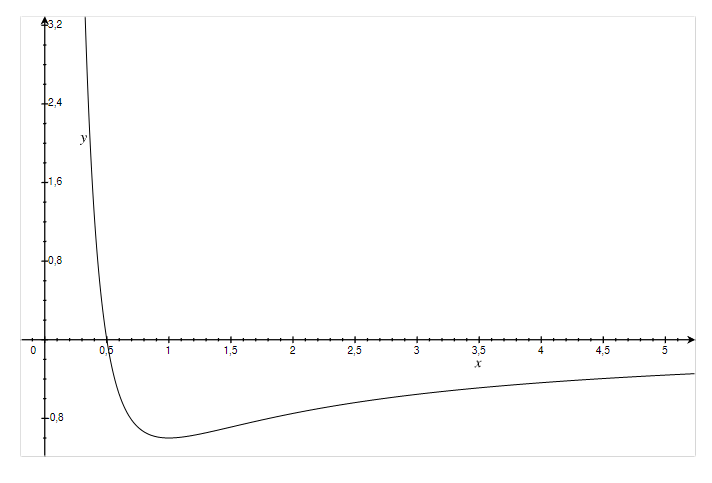
\includegraphics[width=.5\textwidth]{Energiepotentielle_satellite.png}
    \end{figure}
    $Em=Ec+Ep$ comme $Ec>0$ cela implique que les états accessibles : $Em\geq Ep$:
    \begin{itemize}
        \item si $Em=\text{min}(Ep)$: mouvement circulaire
        \item si $\text{min}(Ep)<Em<0$: deux intersections, deux solutions $rmin$ et $rmax$. On a un mouvement qui oscille entre ces deux valeurs.
        \item si $Em>0$, il y a une intersection, mouvement entre $rmin$ et $+\infty$.
    \end{itemize}
    \end{multicols}
\end{frame}

\begin{frame}{\insertsubsection}
    On peut réecrire l'équation sur $\vec{u}_r$: 
    \[\dfrac{d^2u}{d\theta^2}+u=\dfrac{GM}{C^2}\]
    Cette équation a pour solution : 
    \[u = \dfrac{GM}{C^2}+Acos(\theta-\theta_0)\]
    On retrouve alors l'équation d'une conique sur $r$
    \[r=\dfrac{p}{1+e\cos(\theta)}\]
    On peut exprimer l'excentricité en fonction de l'énergie mécanique tel que : 
\begin{equation}
    e = \sqrt{1+\dfrac{2Em}{GMm}}
\end{equation}
Illustrer avec programme python
\end{frame}
% \maketitle
% --------- Sommaire ---------
% \begin{frame}
%     \tableofcontents
% \end{frame}      
% ----------------------------

\end{document}